As was mentioned above, surface extraction is an intermediate step after Topology Optimization and NURBS representation in order to facilitate the conversion. In terms of implementing the surface extraction, we used VTK.

%\subsection{VTK Toolbox}


%The VTK toolbox was used in order to implement the algorithms on our optimized data. It is a heavily object
%oriented toolbox. Our first approach was to use the built in Marching Cubes algorithm,
%nevertheless it did not work with our unstructured grid data. It just works for ImageData and
%PolyData . For structured and unstructured grids the tool to render the isosurface is the \textit{Contour Filter} tool. Unfortunately the documentation does not present which algorithm the tool uses. It
%can be inferred that it is an extended Marching cubes algorithm.

The VTK Toolbox is an open--source tool, providing algorithms for "3D computer graphics, image processing, and visualization" \cite{VTKToolbox}. Among the variety of tools, VTK offers algorithms, allowing us to obtain a surface representation from voxel data. In the midst of these algorithms, we could find Marching Cubes, Dual Contouring and also a Decimation method, which is useful for reducing the data size even further for the NURBS-representation step.


%\subsection{Implementation}
Since \textit{Marching Cubes} algorithm only works with ImageData and PolyData, it is inapplicable to our case of unstructured grid data. For structured and unstructured grids the tool to render the isosurface is the \textit{Contour Filter} tool. Unfortunately, the documentation does not present which algorithm the tool uses. It can be inferred that it is an extended \textit{Marching Cubes} algorithm.
The \textit{Contour Filtering} works fine but the visualization of our data was still not possible
and an intermediate step was needed. We used the \textit{Implicit Modelling} tool which is a filter that
computes the distance from the input geometry to the points of an output structured point set.
This distance function can then be "contoured" to generate new, offset surfaces from the original
geometry. Although this approach allowed the visualisation, some crucial information was lost. In particular, holes are not represented in the final model.  
%It finally allowed visualization but it created one problem. Holes are lost in
%the process.

\begin{figure}
\centering
   \scalebox{0.4}{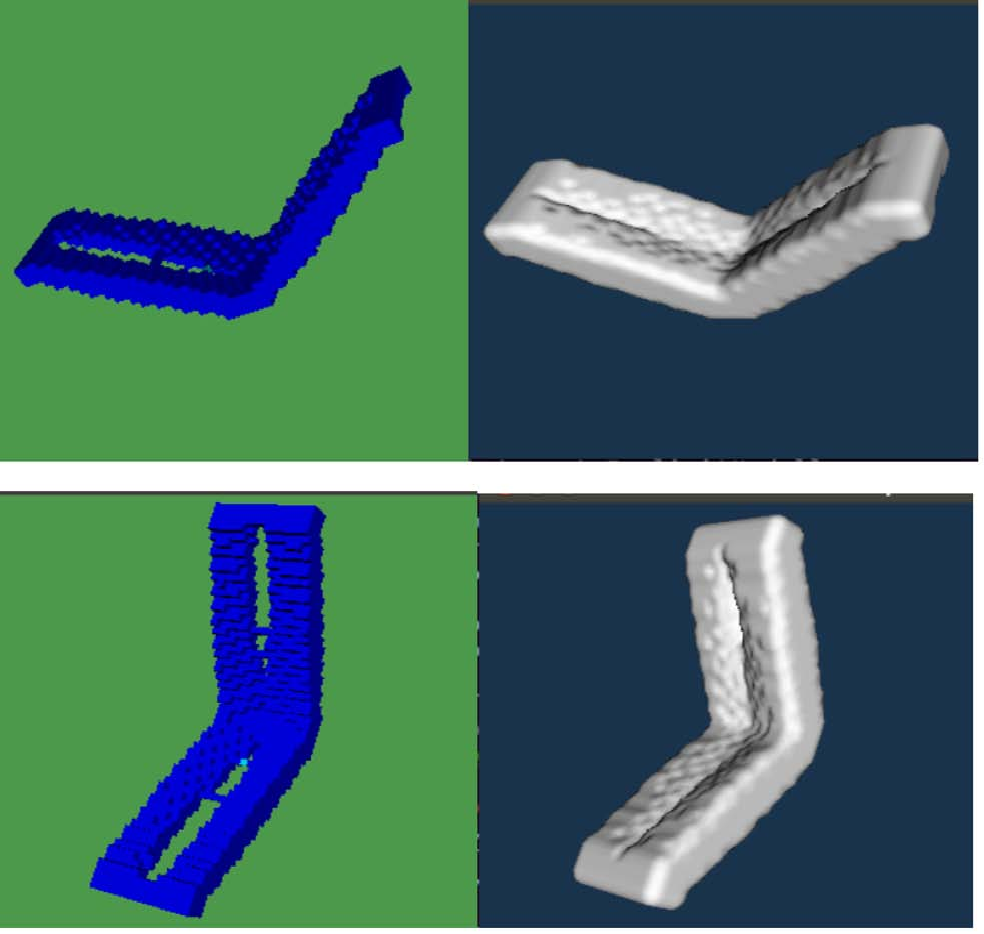
\includegraphics{Pictures/contouring.pdf}}\\
   \caption{Contour Filtering tool after Implicit Modelling}
   \label{fig:contouring}
\end{figure}

A further idea to solve this problem is to first convert the volume data into point data
and only then present it to the \textit{Contour Filtering} tool (\autoref{fig:contouring}).

In order to reduce computational costs of the following \textit{NURBS fitting} process, presented in the next section, we need to create a coarser mesh from the fine one. The number of triangles that represent the
isosurface can be reduced with the \textit{Decimation} tool. A smoothing step is necessary in between
to get the new connections right. The top part of figure \ref{fig:Decimation} shows a 50 \% reduction of the
triangles, a noticeable difference can not be perceived. On the lower part a 90 \% reduction is
obtained, it is nevertheless still difficult to see a difference. Triangle meshes can be easily
coarsened since there are many open source algorithms that simplify the triangles. VTK has the
decimation tool which works for 3D triangle data.

\begin{figure}
\centering
   \scalebox{0.4}{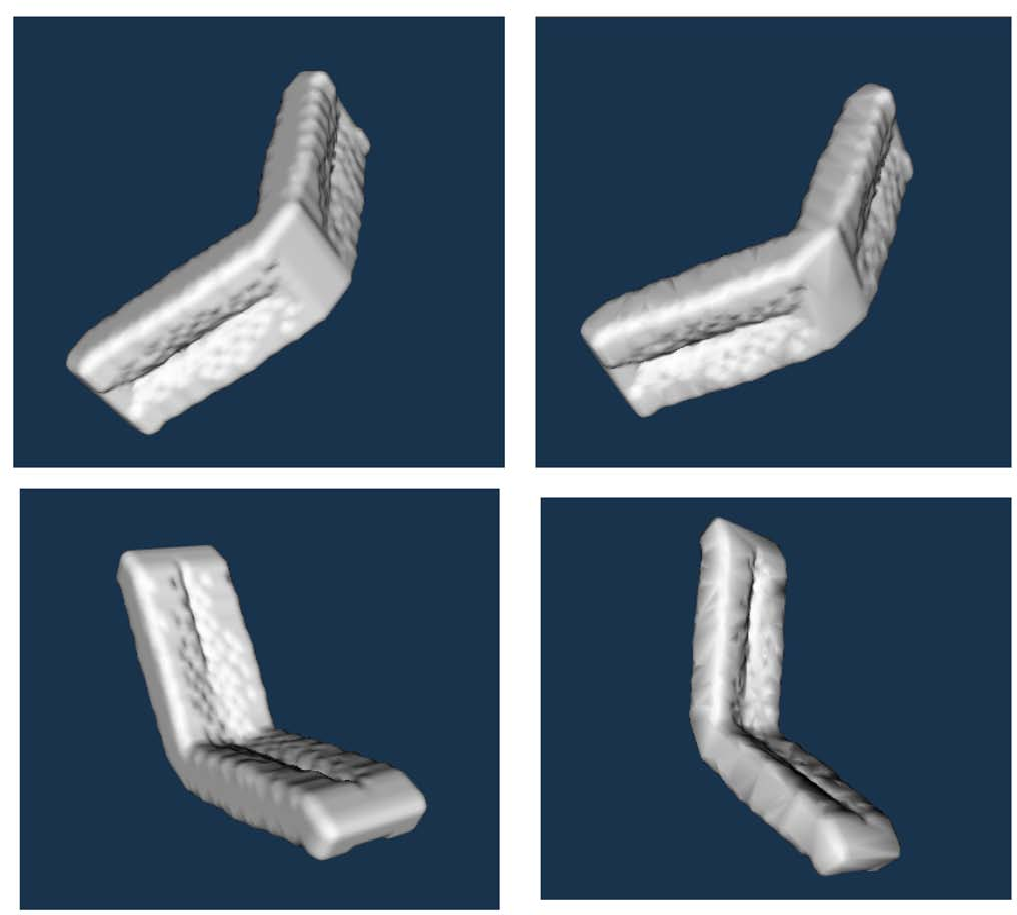
\includegraphics{Pictures/Decimation.pdf}}\\
   \caption{Decimation of triangles. \textit{Top:} 50\% \textit{Lower:} 90\%}
   \label{fig:Decimation}
\end{figure}
